% cite as https://ling.auf.net/lingbuzz/009369

% !TEX TS-program = xelatex
\documentclass[12pt,letterpaper]{article}

%~-- Encoding, fonts (XeLaTeX/LuaLaTeX)~--
\usepackage{fontspec}
\defaultfontfeatures{Ligatures=TeX,Scale=MatchLowercase}
\setmainfont{TeX Gyre Termes}
\setsansfont{TeX Gyre Heros}
\setmonofont{TeX Gyre Cursor}

%~-- Page layout~--
\usepackage[margin=1in]{geometry}
\usepackage[protrusion=true,expansion=false]{microtype}
\usepackage{booktabs}

%~-- Linguistics~--
\usepackage{langsci-gb4e}
\usepackage{tipa}

%~-- Math, symbols~--
\usepackage{amsmath,amssymb}

%~-- Figures ~--
\usepackage{tikz}
\usepackage{pgfplots}
\pgfplotsset{compat=1.18}
\usetikzlibrary{arrows.meta,shapes,positioning,calc}

%~-- Quotes, URLs, colors, links~--
\usepackage{csquotes}
\usepackage[dvipsnames]{xcolor}
\usepackage{hyperref}
\hypersetup{
  colorlinks=true,
  linkcolor=MidnightBlue,
  citecolor=MidnightBlue,
  urlcolor=PineGreen,
  pdfauthor={Brett Reynolds},
  pdftitle={Definiteness and Deitality},
  pdfkeywords={definiteness, article, demonstratives, homeostatic property cluster}
}
\urlstyle{same}

%~-- Lists~--
\usepackage{enumitem}
\setlist{noitemsep, topsep=2pt}

%~--~--~-- - ORCID (linked icon with fallback)~--~--~-- -
\IfFileExists{orcidlink.sty}{%
  \usepackage{orcidlink}%
  \newcommand{\AuthorWithORCID}[2]{##1\,\orcidlink{##2}}%
}{%
  \newcommand{\AuthorWithORCID}[2]{\href{https://orcid.org/##2}{##1}}%
}
\newcommand{\myorcid}{0000-0003-0073-7195}

%~-- Bibliography (BibLaTeX)~--
\usepackage[
  backend=biber,
  bibstyle=unified,    
  citestyle=authoryear-comp, 
  maxcitenames=3,
  maxbibnames=99
]{biblatex}
\addbibresource{refs.bib}

%~-- Macros~--
\newcommand{\Deital}{\textsc{deital}}
\newcommand{\Nondeital}{\textsc{non-deital}}
\newcommand{\Deitality}{\textsc{deitality}}
\newcommand{\Definiteness}{\textsc{definiteness}}
% Upright (non-italic) slash that still allows a break after it
\DeclareRobustCommand{\upslash}{\/\textup{~\slash~}}


%~--~--~-- - Title~--~--~-- -
\title{Definiteness and Deitality in English:\\A Homeostatic Property Cluster Account}
\author{\AuthorWithORCID{Brett Reynolds}{\myorcid}\thanks{I would like to thank Cris Chatterjee for helpful feedback. I used Claude Sonnet 4.5 extensively in drafting and editing this paper with some input from ChatGPT 5 and Gemini 2.5 Pro. I have reviewed and edited all text, and I take full responsibility for all claims and conclusions.}\\[4pt]
Humber Polytechnic \& University of Toronto}
\date{\today}

\begin{document}

\maketitle

\begin{abstract}
I separate the semantic category of \textsc{definiteness} from the structural category of \textsc{deitality} and treat each as a homeostatic property cluster. On the structural side, deitality comprises co-tending properties: distributional restrictions (dispreference as the pivot of existential \textit{there} under neutral prosody, eligibility as the complement of partitive \textit{of}, suitability as hosts for nonrestrictive modification and identificational constructions) and a strong tendency to mark semantically definite referents. On the semantic side, definiteness comprises interpretive properties (identifiability, uniqueness, anaphoric recoverability) and a strong tendency to be marked deitally. The deital cluster is maintained by grammaticalization, acquisition, interactive alignment, prestige selection, and iterated transmission. The definiteness cluster is maintained by discourse-pragmatic mechanisms: common ground management and information structure. Their imperfect alignment yields classic form-meaning mismatches: weak definites, generic definites, and cases where proper names or bare nominals are semantically definite yet morphosyntactically non-deital. This framework explains graded category membership in a principled way and generates falsifiable predictions about how the clusters behave under manipulation.
\end{abstract}

\textbf{Keywords:} definiteness, article, demonstratives, homeostatic property cluster

\newpage
\section{Introduction}\label{sec:intro}

English grammars routinely conflate morphosyntactic form with semantic function. When it comes to definiteness, this conflation creates persistent empirical problems. Tests that target morphosyntax~-- like the definiteness effect in existential \textit{there}~-- are treated as direct probes of uniqueness or familiarity. Meanwhile, semantic heuristics~-- like asking whether it makes sense to say \textit{which one?}~-- are used to define grammatical categories. The result is a theoretical tangle where neither form nor meaning gets a clean characterization.

I propose a radical decoupling. The structural category~-- which I call \Deitality{}~-- is defined by a cluster of distributional properties that co-occur in English determiners. The semantic category \Definiteness{} is defined by a distinct cluster of interpretive properties related to referent identifiability. Deitality is morphosyntactic but often semantically definite; definiteness is semantic but often morphosyntactically deital. The correlation is strong. The identity is absent. 

This misalignment produces well-known puzzles. So-called ``weak definites" like \textit{go to the hospital}~-- I retain the label though the analysis here treats them as deital but indefinite~-- combine deital morphology with semantically indefinite reference. ``Generic definites" like \textit{The tiger is endangered} are deital but involve kind reference rather than individual-level definiteness. And proper names are semantically definite yet morphosyntactically non-deital. These are classic cases of form-function mismatch \parencite{FrancisMichaelis2003}: the morphosyntactic and semantic categories systematically come apart.

The theoretical apparatus comes from the philosophy of science. I model both deitality and definiteness as \textsc{homeostatic property clusters} or HPCs \parencite{Boyd1991,Boyd1999}. An HPC kind is characterized not by necessary and sufficient conditions but by a family of properties that co-tend because of underlying causal mechanisms. No single property is required; membership is graded; boundaries are fuzzy. What makes the category coherent is that the properties stabilize together over time.

Each cluster comprises properties from both morphosyntactic and semantic domains, but the mechanisms maintaining them differ. For deitality, five mechanisms operate at distinct timescales: grammaticalization creates the cluster phylogenetically when demonstratives become articles; acquisition filters it ontogenetically as each generation learns it; interactive alignment stabilizes it microgenetically in real-time conversation; prestige selection shapes it sociogenetically across communities; iterated transmission filters it phylogenetically across generations. For definiteness, the mechanisms are discourse-pragmatic: common ground management, bridging, and topic continuity create correlations among identifiability, uniqueness, and anaphoric tracking. The clusters overlap substantially~-- most deital marking appears on definite referents~-- but the distinct mechanisms allow systematic dissociations.

The payoff is both empirical and theoretical. Empirically, the HPC framework explains why deitality and definiteness align without being identical, why weak and generic definites exist, and why proper names pattern as they do. It also generates falsifiable predictions about how the clusters respond to prosodic manipulation, specificity forcing, and dialectal variation. Theoretically, it offers a principled way to embrace graded category membership: categories can have prototypical members and gradient edges while remaining real and explanatorily useful.

The paper proceeds as follows. Section~\ref{sec:hpc} introduces the HPC framework and justifies its application to grammatical categories. Section~\ref{sec:semantic} characterizes definiteness as a semantic cluster. Section~\ref{sec:diagnostics} develops the diagnostics for deitality as morphosyntactic tests. Section~\ref{sec:mechanisms} identifies the homeostatic mechanisms maintaining the deital cluster and derives empirical predictions. Section~\ref{sec:cases} applies the framework to weak and generic definites. Section~\ref{sec:objections} addresses edge cases and objections. Section~\ref{sec:conclusion} concludes.

\section{Homeostatic property clusters: A framework for messy categories}\label{sec:hpc}

The proposal to treat grammatical categories as homeostatic property clusters requires justification. The HPC framework originated in philosophy of biology to solve the species problem \parencite{Boyd1991,Boyd1999}. I'll sketch the biological motivation, extract the core theoretical machinery, and then show why it applies to linguistic categories.

\subsection{The species problem and its solution}

For centuries, biologists sought an essentialist definition of species: a set of necessary and sufficient conditions for membership. Traditional candidates included morphological similarity, ability to interbreed, and shared ancestry. Each definition failed. Ring species can interbreed with adjacent populations but not with distant ones. Asexually reproducing organisms don't interbreed at all. Morphologically similar organisms can be reproductively isolated. The natural world resisted crisp boundaries \parencite{Mayr1942}.

Boyd's solution was to reject essentialism entirely. A species isn't defined by a single property or fixed set of properties. Instead, it's characterized by a \textit{cluster} of properties~-- morphological, genetic, behavioural~-- that co-occur more often than chance would predict. What makes this clustering stable is a set of causal mechanisms: gene flow within the population, developmental constraints, shared ecological niche, natural selection. These mechanisms are \textit{homeostatic} because they maintain the integrity of the cluster even when individual members lack some properties.

Three features define an HPC kind. First, there's a \textit{contingent property cluster}: a family of properties that statistically co-occur. No single property is necessary; no set is sufficient. Second, the clustering is causally sustained by \textit{homeostatic mechanisms}: underlying processes that ensure the presence of some properties tends to favor others. Third, the mechanisms aren't perfect, which produces \textit{imperfect homeostasis}: graded membership, prototype effects, and fuzzy boundaries.

The epistemic justification comes from Boyd's accommodation thesis \parencite{Boyd1991,Boyd1999}. A category is a natural kind if treating it as such allows scientists to formulate reliable generalizations and explanations. The category is ``natural" not because it mirrors a pre-existing Platonic structure but because it's projectable: it supports successful induction and prediction.

\subsection{Why grammatical categories need this framework}

The parallel to linguistics is direct. Just as biologists sought an essence for species, linguists have sought one for definiteness. Decades of research have tried to define ``definite noun phrase" by semantic essence~-- uniqueness \parencite{Russell1905,Hawkins1978} or familiarity \parencite{Christophersen1939,Heim1982}. But counterexamples proliferate. Weak definites like \textit{listen to the radio} use \textit{the} without uniqueness \parencite{CarlsonSussman2005,AguilarGuevaraZwarts2010}. Generic definites like \textit{The lion is noble} refer to kinds, not individuals \parencite{Carlson1977,Krifka2004}. Cross-linguistically, definite articles appear in contexts where their semantic contribution seems redundant or absent \parencite{Lyons1999}.

These aren't peripheral exceptions. They're systematic patterns that suggest the category lacks a simple essence. The attempt to define a morphosyntactic object~-- the class of noun phrases marked with definite morphology~-- using purely semantic criteria has produced a category that doesn't align with the empirical facts.

The HPC framework offers a way forward. We can characterize both deitality and definiteness as property clusters maintained by distinct causal mechanisms. The strong correlation between them is real and causally grounded, but the clusters can and do come apart in systematic ways \parencite{FrancisMichaelis2003}. The subsequent sections develop this account: §\ref{sec:semantic} characterizes the definiteness cluster, §\ref{sec:diagnostics} establishes the deitality cluster through convergent diagnostics, and §\ref{sec:mechanisms} identifies the homeostatic mechanisms maintaining both.

This move has precedent. Prototype theory in cognitive linguistics has long recognized that categories have graded structure \parencite{Rosch1978,Lakoff1987}. But prototype theory often lacks a causal story about why certain properties cluster. The HPC framework provides that story. It's not just that some members are ``better examples" than others. It's that causal mechanisms actively maintain the clustering while allowing for variation at the edges.

The HPC framework has already been applied to linguistic phenomena. \textcite{Miller2021} argues that word-kinds like \textit{table} and \textit{Paris} are HPCs, defined by clusters of phonological, orthographic, and semantic properties maintained by cognitive and social mechanisms. The present proposal extends this approach from lexical ontology to grammatical categories. Where Miller asks what makes tokens instances of the same word-kind, I ask what distinguishes deital from non-deital determiners~-- why \textit{the}, \textit{this}, and genitives pattern together distributionally while \textit{a}, \textit{some}, and \textit{many} form a contrasting cluster.

\section{Definiteness as a semantic property cluster}\label{sec:semantic}

Before characterizing deitality, I need to clarify what definiteness IS~-- semantically and pragmatically~-- so it's clear what deitality ISN'T. The literature presents two major traditions: uniqueness theories and familiarity theories. Rather than adjudicating between them, I'll argue that both capture important properties in the definiteness cluster.

Uniqueness theories originate with Russell \parencite{Russell1905}. A definite description \textit{the F} presupposes that exactly one entity satisfies \textit{F} in the contextually relevant domain. Later work refined this to allow pragmatic restriction: uniqueness holds relative to a ``P-set" or shared frame of reference \parencite{Hawkins1978}. This approach handles ``larger situation" uses like \textit{the sun} and anaphoric uses where prior discourse has narrowed the context to a single salient entity.

Familiarity theories stem from Christophersen and were formalized by Heim \parencite{Christophersen1939,Heim1982}. Definite noun phrases are subject to a familiarity condition: they must refer to an entity already established in the discourse model. Indefinites, by contrast, introduce new referents. This framework excels at explaining discourse anaphora, where a definite's felicity depends directly on having a linguistic antecedent.

Both theories have problems. Familiarity isn't necessary~-- \textit{the first person on Mars} can be used felicitously even when the referent is discourse-new. Uniqueness isn't sufficient~-- in contexts with two familiar but non-unique entities, neither \textit{the N} works smoothly. And weak definites challenge both: \textit{go to the hospital} uses \textit{the} when the hospital is neither uniquely specified nor discourse-familiar \parencite{Abbott2004,Birner2013}.

I propose that uniqueness and familiarity are both properties in the definiteness cluster, along with anaphoric recoverability and, more broadly, identifiability. These properties co-tend because of discourse-pragmatic mechanisms: common ground management makes unique entities easier to track; anaphoric devices rely on familiarity; topics bias toward identifiable referents. But the co-occurrence is statistical, not absolute.

This explains the theoretical debate. Uniqueness and familiarity theorists aren't discovering competing essences. They're mapping different regions of the same property cluster. The clusters overlap heavily~-- a discourse-old, unique referent satisfies both~-- but they dissociate in predictable ways. Weak definites have identifiability without token-level uniqueness. Cataphoric definites have uniqueness without prior familiarity. The semantic notion of definiteness is itself an HPC.

What matters for present purposes is this: definiteness is a property cluster centred on interpretation~-- how referents are mentally represented and tracked in discourse. The core properties are identifiability, uniqueness, and anaphoric recoverability. But the cluster also includes a morphological tendency: definite referents are strongly associated with deital marking. This association is maintained by discourse efficiency and grammaticalization history, creating substantial overlap with the deitality cluster. The next sections establish the deitality cluster through convergent diagnostics (§\ref{sec:diagnostics}) and identify the distinct mechanisms maintaining it (§\ref{sec:mechanisms}). The imperfect alignment between clusters~-- cases where definiteness and deitality dissociate~-- is the focus of §\ref{sec:cases}.

\section{Diagnostics for deitality}\label{sec:diagnostics}

I characterize deitality as a structural property cluster whose core comprises distributional restrictions but also includes a strong tendency to mark semantically definite referents. This section develops four core diagnostics that target the distributional restrictions: existential \textit{there}, partitive \textit{of}, identificational hosting, and \textit{one}-substitution. These diagnostics establish the morphosyntactic spine of the cluster; §\ref{sec:mechanisms} explains how grammaticalization and other mechanisms link this spine to definiteness-marking. Each diagnostic is construction-general, targets the determiner itself, and admits controllable neutralizations.

\subsection{Existential \textit{there}}

The definiteness effect in existential \textit{there} constructions is well-documented \parencite{Milsark1977,McNally2011}. Under neutral prosody, deital determiners resist the pivot position:

\ea 
\label{ex:there-neutral}
    \ea \textit{\textsuperscript{*}There is the key on the table.}
    \ex \textit{\textsuperscript{*}There are those books I mentioned.}
    \ex \textit{There is a key on the table.} (non-deital, acceptable)
    \z
\z

The effect is sensitive to prosody: list/presentational intonation can license otherwise dispreferred pivots \parencite{BirnerWard1998}:

\ea 
\label{ex:there-list}
    \ea \textit{There's THAT book again.}
    \ex \textit{Well, there's the KEYS, the wallet...}
    \z
\z

\textbf{note: Cris Chatterje asks ``are you sure that's an expletive there at the beginning as opposed to the preposition? I'm finding it difficult to give it a presentational reading."}

I treat this as a controllable neutralization: under neutral prosody, deital determiners resist the pivot position; marked prosody can ameliorate the effect. The diagnostic is therefore calibrated to neutral prosody.

\textbf{Important calibration}: This diagnostic~-- and indeed each diagnostic in this section~-- is calibrated to \textit{neutral prosody and non-narrative frames}. Specialized constructions like narrative-presentational \textit{There was this guy...} have their own licensing conditions (see §\ref{sec:cases}) and don't constitute counterevidence to the basic distributional pattern.

\subsection{Partitive \textit{of}}

In true partitive constructions~-- \textit{X of Y} with subset semantics~-- the \textit{Y} complement must be definite-like \parencite{Barker1998,Hoeksema1996}:

\ea 
\label{ex:part-good}
    \ea \textit{Two\upslash several\upslash many of the students left.}
    \ex \textit{Two\upslash several\upslash many of these\upslash my students left.}
    \z
\z

\ea 
\label{ex:part-bad}
*\textit{Two\upslash several\upslash many of some students left.}
\z

This selectional restriction is robust and not ameliorated by prosody. Attempts to use weak \textit{Y} are either rejected outright or reanalyzed as measure/fraction constructions (\textit{half of a cake}), which have different semantics.

It's the \textit{Y} slot that matters. Elements in \textit{X}~-- including quantifiers like \textit{all} or \textit{both} when they appear as modifiers~-- are irrelevant to this diagnostic.

\subsection{Identificational hosting}

Deital determiners are preferred hosts for nonrestrictive modification, topics, and specificational subjects. Weak determiners are degraded unless coerced to specific readings \parencite{Lambrecht1994}:

\ea 
\label{ex:host-good}
    \ea \textit{The\upslash this\upslash John's book, which I bought yesterday, is excellent.}
    \ex \textit{As for the\upslash this\upslash John's report, I've filed it.}
    \ex \textit{The culprit is John.}
    \z
\z

\ea 
\label{ex:host-bad}
    \ea \textsuperscript{??}\textit{A book, which I bought yesterday, is excellent.}
    \ex \textsuperscript{??}\textit{As for a report, I've filed it.}
    \ex \textsuperscript{??}\textit{A culprit is John.}
    \z
\z

The degradation correlates with information structure. Identificational constructions presuppose that the referent is already salient or identifiable to the hearer. Weak indefinites introduce new referents and clash with this presupposition.

\subsection{\textit{One}-substitution}

Non-deital determiners freely allow bare anaphoric \textit{one} across clauses:

\ea 
\label{ex:one-weak}
\textit{I bought a red pen and you bought one too.}
\z

Deital packages resist bare \textit{one} in the same configuration:

\ea 
\label{ex:one-strong}
*\textit{I bought the\upslash this\upslash my red pen and you bought one too.}
\z

Determiner + \textit{one} (\textit{this one}, \textit{the one}) is grammatical but represents a different construction: \textit{one} is a noun with its own determiner, not a determinative phrase in fused-determiner--head function \parencite[332--333]{HuddlestonPullum2002}. I exclude this construction from the diagnostic.

This test is narrower than the others and more subject to dialectal variation. I treat it as a corroborating cue rather than a primary diagnostic.

\subsection{Summary: Converging evidence for a property cluster}

These four diagnostics converge on a morphosyntactic profile. Prototypical deital determiners resist existential pivots, license partitive \textit{Y}, host identificational constructions naturally, and disprefer bare \textit{one}-substitution. Prototypical non-deital determiners show the opposite pattern. No single diagnostic defines the cluster. No diagnostic has metaphysical privilege; no property is necessary, no set sufficient. What matters is convergence across multiple independent tests~-- the homeostatic pattern that essentialist accounts cannot capture.

In applying the tests (see Appendix~\ref{sec:inventory}), many determinatives show partial cluster membership. Items like \textit{each}, \textit{every}, \textit{all}, and \textit{both} resist existential pivots (patterning deitally) but fail other diagnostics (patterning non-deitally). This is exactly what the HPC framework predicts: graded membership reflecting different degrees of property clustering. The diagnostic convergence defines a space where \textit{the} and demonstratives occupy the prototypical center while other items show gradient participation.

This property pluralism is central to the HPC framework: just as biological species are characterized by multiple co-tending traits (morphology, genetics, behaviour) with none metaphysically prior, deitality is characterized by multiple co-tending distributional properties with none foundational. The diagnostics are equally valid cues to cluster membership.

That said, not all diagnostics are equally reliable in practice. Some show more cross-linguistic stability; some resist dialectal variation better; some apply more broadly. The \textit{one}-substitution test, for instance, is more subject to dialectal variation than partitive \textit{Y}-selectivity, making it a less robust probe in fieldwork. But both target equally real properties of the deital cluster. These are empirical differences in diagnostic utility, not metaphysical differences in the properties themselves.

Importantly, these diagnostics target distributional behaviour rather than semantic contribution. This doesn't mean the deital cluster lacks semantic properties~-- it correlates strongly with identifiability, wide scope, and anaphoric tracking. But these semantic tendencies are properties \textit{within} the cluster, not necessary conditions for membership. A determiner can be deital while contributing non-prototypical semantics: weak definites lack token-level uniqueness; generic definites refer to kinds. The morphosyntactic profile is what remains stable across this semantic variation.

Section~\ref{sec:mechanisms} identifies the homeostatic mechanisms that create and maintain this diagnostic clustering.

\section{Homeostatic mechanisms maintaining the deital cluster}\label{sec:mechanisms}

The central claim of the HPC framework is that property clustering isn't accidental. It's causally sustained by homeostatic mechanisms. For deitality, five mechanisms operate at distinct timescales to maintain both the distributional restrictions (partitive licensing, \textit{there}-resistance, hosting, \textit{one}-blocking) and the strong correlation with definiteness-marking: grammaticalization creates the cluster; acquisition, interactive alignment, prestige selection, and iterated transmission maintain it across individuals, conversations, communities, and generations. For definiteness, the mechanisms are discourse-pragmatic: information structure and common ground management create correlations among identifiability, uniqueness, and anaphoric recoverability, while also reinforcing the tendency for definite referents to be marked deitally.

The previous section established four diagnostic properties that converge to define the deital cluster. This section identifies five homeostatic mechanisms operating at distinct timescales, shows how they interact to maintain that cluster, and derives falsifiable predictions about synchronic grammar.

\subsection{Five mechanisms across timescales}\label{subsec:five-mechanisms}

\subsubsection{Grammaticalization: Creating the cluster (phylogenetic, centuries)}\label{subsec:gram}

Cross-linguistically, definite articles arise primarily from demonstratives \parencite{Greenberg1978,Diessel1999}. As a demonstrative grammaticalizes~-- weakening phonologically and broadening functionally~-- it doesn't shed its distributional properties. It drags them along.

Demonstratives inherently show many properties of the deital cluster. They're deictic, which makes them poor candidates for introducing discourse-new referents (hence resistance to existential \textit{there}). They're referential and often presuppositional, which makes them natural hosts for identificational constructions. They pattern with definites in partitive constructions cross-linguistically.

When a demonstrative becomes an article, these distributional tendencies persist. The resulting article inherits the morphosyntactic frame even as its semantic function generalizes from pure deixis to broader identifiability marking. This is property dragging: grammaticalization preserves formal behaviour while semantic function shifts.

English \textit{the} shows exactly this pattern. Historically derived from a demonstrative, it resists existential pivots, licenses partitive \textit{Y}, and hosts identificational constructions~-- all properties traceable to its deictic source. Weak definites, where \textit{the} appears without uniqueness, represent cases where the morphosyntactic frame has outlived the original semantic restriction.

The grammaticalization account predicts that items sharing a deictic source should share distributional properties. English offers phonological evidence for this prediction. All /ð/-initial determinatives are deital: \textit{the}, \textit{this}, \textit{that}, \textit{these}, \textit{those}. This clustering isn't universal~-- other function words like \textit{then}, \textit{than}, \textit{though} begin with /ð/ without being determinatives, and many deital items like genitives lack it entirely. But within the determinative class, /ð/ marks a family of historically related forms, all derived from Germanic demonstratives. The phonological property clusters with the distributional ones because both reflect common ancestry. Property dragging operates on bundles: when demonstratives grammaticalize, they carry along not just distributional behaviour but phonological shape.

\subsubsection{First language acquisition: Filtering the hypothesis space (ontogenetic, childhood)}

The grammatical system must be acquired by each new generation. The acquisition process acts as a filter: only stable, learnable patterns survive transmission.

Children acquire deital determiners early, often overgeneralizing \textit{the} to contexts where adults use \textit{a} \parencite{Maratsos1976,RozendaalBaker2008}. This isn't semantic confusion. It's structural success. Children identify a high-frequency form (\textit{the}) plus its distributional frame~-- appears with familiar referents, resists existential contexts, patterns with genitives~-- and apply it broadly before refining the semantic conditions.

Critically, they acquire the morphosyntactic cluster before mastering the full semantic range. They know \textit{the} appears in certain structural positions (determiner slot, partitive complement) before they know exactly when referents count as unique or familiar. This creates a bootstrapping dynamic: the distributional frame helps learners infer semantic function, and vice versa.

This acquisitional filtering maintains the cluster's stability. Each generation re-creates the deitality category based on distributional evidence. The property cluster~-- pivot resistance, partitive licensing, identificational hosting~-- is learned as a package, not as independent facts. When children overgeneralize, they extend the entire package. When they refine, they adjust semantic conditions while preserving the morphosyntactic frame.

\subsubsection{Interactive alignment and repair: Real-time stabilization (microgenetic, seconds to minutes)}

In conversation, speakers converge automatically on syntactic frames and prune misalignments through immediate repair \parencite{PickeringGarrod2004}. When a speaker produces a deital determiner in a dispreferred context~-- say, \textit{There's the problem} under neutral prosody~-- hearers flag the anomaly either through explicit correction or through subtle cues (hesitation, clarification requests). This real-time feedback loop stabilizes the distributional patterns within individual interactions.

The mechanism operates largely below conscious awareness. Speakers don't explicitly reason about partitive selectional restrictions; they simply experience discomfort when hearing \textit{*two of some students} and either repair the utterance or signal non-comprehension. Over thousands of conversational exchanges, this microgenetic pruning reinforces the property cluster by penalizing violations and rewarding canonical patterns.

\subsubsection{Prestige-weighted selection: Social stratification (sociogenetic, decades)}

Variants associated with high-status speakers spread faster through communities \parencite{labov2001,eckert2000}, pushing some constructions toward categorical bans while allowing sociolinguistic stratification to persist at gradient margins. 

For deitality, this mechanism explains why some weak definite frames (British \textit{in hospital}) become dialectally entrenched while others never stabilize. Prestige dynamics can override frequency: highly frequent non-standard patterns (\textit{them books} in some dialects) remain marked because standard \textit{those books} carries social prestige. Conversely, low-frequency prestige forms can resist elimination.

The mechanism doesn't create the deital cluster~-- grammaticalization and acquisition do that~-- but it shapes which variants survive community transmission and which get filtered out. This explains why structural bans often correlate with social evaluation even when the underlying constraint is cognitive or morphosyntactic.

\subsubsection{Iterated cultural transmission: Multi-generational filtering (phylogenetic, generations)}

The transmission bottleneck amplifies learnability biases and filters out mappings that exceed processing or memory constraints \parencite{Kirby2014}. Each generation learns the language from finite input, necessarily discarding patterns that are too complex, too rare, or too inconsistent to acquire reliably.

This multi-generational ratchet explains why structural bans converge across dialects even as surface patterns diverge. Determiner extraction (\textit{*Which did you buy car?}) is categorically rejected in all English dialects because the underlying constraint~-- no stranding of determiners~-- is simple, learnable, and stable under transmission. Weak definite frames, by contrast, show dialectal variation because they're conventionalized idioms: learnable but not structurally forced.

Iterated transmission also explains the phonological clustering noted in §\ref{subsec:gram}. The /ð/-initial family persists not because of any functional advantage but because the phonological pattern is stable under transmission. Children acquiring English identify the cluster and reproduce it, generation after generation.

\subsection{Causal architecture: How mechanisms interact}


Figure~\ref{fig:deital-homeostasis} schematizes how the five mechanisms stabilize the deital property cluster. Grammaticalization creates the initial bundle; four mechanisms maintain it simultaneously at different timescales.

\begin{figure}[htbp]
\centering
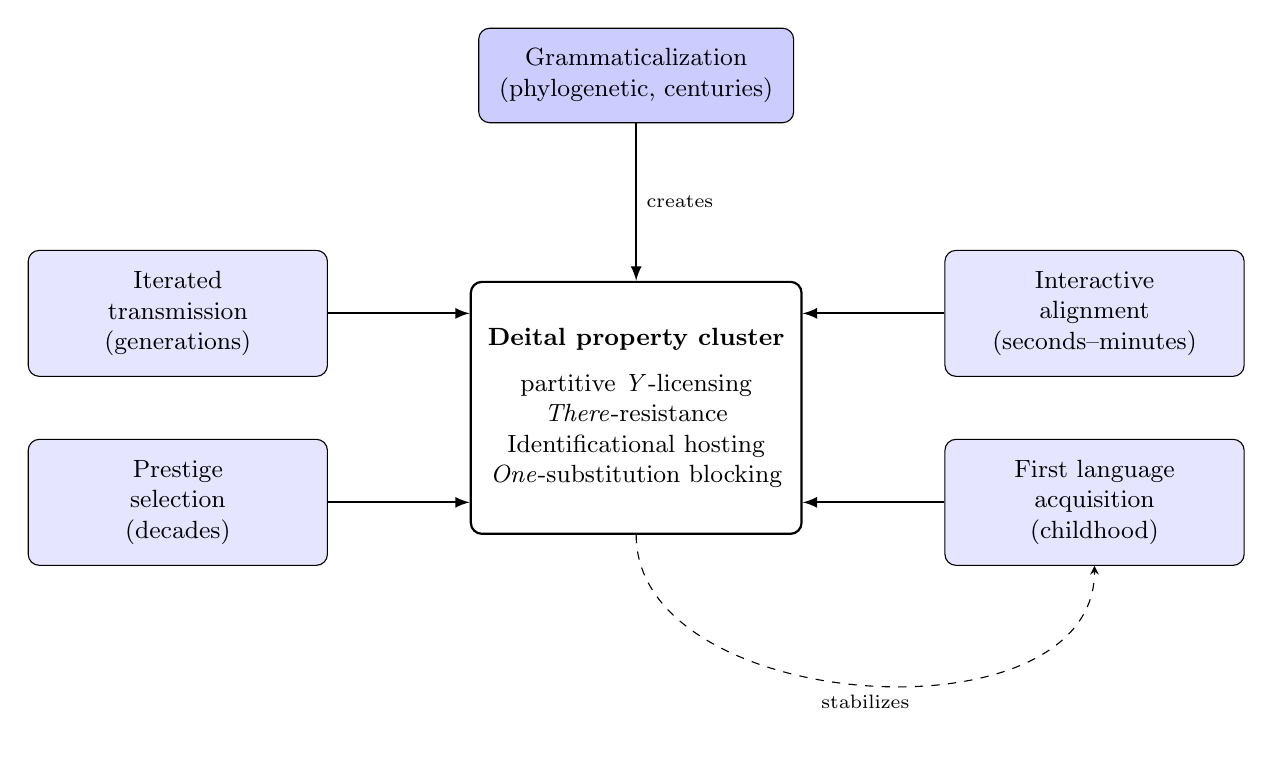
\begin{tikzpicture}[
  font=\small,
  node distance = 10mm and 18mm,
  origin/.style = {rectangle, draw, rounded corners,
                   minimum width=40mm, align=center, text depth=0.5ex,
                   fill=blue!20, minimum height=12mm},
  mech/.style = {rectangle, draw, rounded corners,
                 minimum width=38mm, align=center, text depth=0.5ex,
                 fill=blue!10, minimum height=16mm},
  cluster/.style = {rectangle, draw, rounded corners, thick,
                    minimum width=42mm, minimum height=32mm, align=center},
  prim/.style = {->, >=latex, thick},
  sec/.style = {->, dashed, >={stealth}}
]

% Top: Origin mechanism
\node[origin] (gram) at (0,0) {Grammaticalization\\(phylogenetic, centuries)};

% Middle: Property cluster being maintained
\node[cluster, below=20mm of gram] (props) {
  \textbf{Deital property cluster}\\[2mm]
  \small
  partitive \textit{Y}-licensing\\
  \textit{There}-resistance\\
  Identificational hosting\\
  \textit{One}-substitution blocking
};

% Left: Maintenance mechanisms
\node[mech, left=of props, yshift=12mm] (iter) {Iterated\\transmission\\(generations)};
\node[mech, left=of props, yshift=-12mm] (prestige) {Prestige\\selection\\(decades)};

% Right: Maintenance mechanisms
\node[mech, right=of props, yshift=12mm] (align) {Interactive\\alignment\\(seconds--minutes)};
\node[mech, right=of props, yshift=-12mm] (acq) {First language\\acquisition\\(childhood)};

% Grammaticalization creates the bundle
\draw[prim] (gram.south) to node[right, font=\scriptsize] {creates} (props.north);

% Four maintenance mechanisms (all simultaneous)
\draw[prim] (iter.east) to (props.west |- iter.east);
\draw[prim] (prestige.east) to (props.west |- prestige.east);
\draw[prim] (align.west) to (props.east |- align.west);
\draw[prim] (acq.west) to (props.east |- acq.west);

% Feedback: stable cluster enables acquisition
\draw[sec, rounded corners] (props.south) to [out=270, in=270] 
  node[below, font=\scriptsize] {stabilizes} (acq.south);

\end{tikzpicture}
\caption{Homeostatic mechanisms stabilizing the deital property cluster. Grammaticalization (top) created the initial property bundle through demonstrative-to-article pathways. Four mechanisms maintain the cluster simultaneously at different timescales: iterated transmission filters for learnability across generations; prestige-weighted selection shapes social distribution over decades; interactive alignment maintains patterns in real-time conversation; first language acquisition reproduces the cluster in each generation. The cluster's stability feeds back to enable successful acquisition (bottom), creating a self-reinforcing cycle. Solid arrows show primary causation; dashed arrow shows feedback.}
\label{fig:deital-homeostasis}
\end{figure}

The architecture reveals why deitality is stable yet variable. Grammaticalization creates the initial property bundle through demonstrative-to-article pathways. Acquisition filters this input, preserving only learnable patterns. Interactive alignment maintains the cluster in real-time conversational practice. Prestige selection shapes which variants survive socially. Iterated transmission eliminates patterns that can't survive the multi-generational bottleneck.

The feedback loop at the bottom of Figure~\ref{fig:deital-homeostasis} is critical. Once the cluster stabilizes, it becomes the target of acquisition: children learn the stable pattern, which reinforces its stability in the next generation. This positive feedback explains why the deital cluster persists despite constant pressure from analogy, frequency effects, and contact-induced change.

\subsection{Why deitality and definiteness correlate imperfectly}\label{subsec:autonomy}

Grammaticalization and acquisition explain why deitality exists as a stable morphosyntactic cluster. But why does it correlate with definiteness? And why isn't the correlation perfect?

The correlation arises because the deictic sources of articles were themselves sensitive to information structure. Demonstratives mark salient, often identifiable referents. As they grammaticalize, this functional tendency becomes conventionalized. Speakers and hearers coordinate on using the article for identifiable referents because that's what the form conventionally signals.

This coordination is maintained by communicative efficiency. Speakers remember high-frequency pairings~-- \textit{the} plus unique/familiar referents~-- and hearers expect them. When speakers violate expectations, hearers accommodate by adjusting their domain of evaluation, coercing to specific readings, or reanalyzing the structure. This creates a stable equilibrium where form and function align statistically.

But the correlation isn't perfect because grammaticalization preserves formal residue. Weak definites like \textit{take the bus} reflect conventionalized frames where \textit{the} appeared because of institutional or habitual association, and that morphosyntactic pattern persisted even as the semantic contribution remained indefinite. The distributional residue~-- appears with \textit{the}, resists modification, allows only certain verb-noun pairs~-- is the grammaticalized fossil of a construction, not of a semantic feature.

The mismatch also reflects constructional autonomy. Once a morphosyntactic pattern is established, it can be recruited for new functions. \textit{The poor}, \textit{the unknown} as fused modifier--head NPs use \textit{the} to signal definiteness at the constructional level, not the lexical level. The frame itself becomes meaningful, semi-independent of the article's core function.

\subsection{Projectability tests: Evidence that deitality is a natural kind}

An HPC kind must support inductive and explanatory practices. Deitality passes several tests showing it functions as a projectable category.

\subsubsection{Test 1: Cross-construction generalization}

Knowing that a speaker rejects *\textit{There's the solution} (under neutral prosody) allows reliable prediction that they'll also reject:
\begin{itemize}
\item *\textit{There are those books you wanted} (neutral prosody)
\item *\textit{Two of some students passed} (partitive with weak \textit{Y})
\item \textsuperscript{??}\textit{A book, which cost \$50, was excellent} (indefinite hosting nonrestrictive)
\end{itemize}
This projectability extends across the four core diagnostics. The violations all involve configurations that clash with deital distributional requirements: existential pivots under neutral prosody, non-deital partitive complements, indefinite hosts for identificational constructions.

The generalization works because the deital cluster is causally unified. It's not an arbitrary list of banned sentences; it's a family of constraints flowing from the same underlying property bundle. Once a speaker has acquired the cluster, they project it to novel structures automatically.

\subsubsection{Test 2: Dialectal pattern prediction}

If deitality is a genuine kind maintained by the mechanisms in §\ref{subsec:five-mechanisms}, then dialectal variation should follow principled patterns. Specifically:

\textbf{Convergence prediction}: All dialects should converge on properties maintained by acquisition and iterated transmission (universal cognitive constraints).

\textbf{Divergence prediction}: Dialects should diverge on properties shaped by prestige selection and constructional conventionalization (social and idiomatic factors).

The data confirm both predictions. All English dialects reject determiner stranding (\textit{*Which did you buy car?}), showing convergence on a core structural constraint. But dialects vary on weak definite frames (\textit{in hospital} vs. \textit{in the hospital}), showing divergence on conventionalized idioms.

Cross-linguistic data extend the pattern. Languages with demonstrative-derived articles (French \textit{le}, German \textit{der}, Greek \textit{o}) show similar partitive restrictions and existential resistance. Languages with articles from other sources or no articles show different patterns. The correlation between grammaticalization pathway and distributional profile supports treating deitality as a causally grounded kind, not a stipulated list.

\subsubsection{Test 3: Acquisitional trajectory prediction}

If the mechanisms in §\ref{subsec:five-mechanisms} are correct, child language acquisition should show specific developmental asymmetries:

\textbf{Prediction 3a}: Children should master distributional restrictions (where \textit{the} can appear syntactically) before semantic restrictions (when to use it pragmatically).

\textbf{Prediction 3b}: Children should overgeneralize \textit{the} to semantically inappropriate contexts while respecting morphosyntactic constraints.

\textbf{Prediction 3c}: Children should show earlier mastery of syntactic constraints (partitive \textit{Y}-selectivity) than discourse-pragmatic ones (existential pivot resistance under neutral prosody).

Existing acquisition data support 3a and 3b \parencite{Maratsos1976,RozendaalBaker2008}. Prediction 3c remains to be tested systematically, but the logic is clear: syntactic selectional restrictions don't yield to prosodic manipulation (see §\ref{sec:prosody}), so children can't use prosody as a repair strategy. Discourse-pragmatic constraints do yield to prosody, giving children a fallback. The predicted asymmetry follows from the different causal bases of the constraints.

\subsection{Falsifiable predictions about synchronic grammar}\label{sec:predictions}

The homeostatic mechanisms generate specific predictions about how the synchronic grammar behaves under manipulation. These predictions distinguish the HPC account from alternatives by targeting the interaction between morphosyntax, prosody, semantics, and development. Each prediction is falsifiable and testable.

\subsubsection{Prediction 1: Prosodic manipulation dissociation}\label{sec:prosody}

\textbf{Claim}: Prosody should selectively rescue existential pivots but not partitive complements.

\textbf{Logic}: Prosody can rescue what discourse creates; prosody cannot rescue what syntax demands. Existential pivots yield to marked intonation because their constraint is discourse-pragmatic~-- neutral prosody enforces information-structural requirements, but contrastive or list prosody can override those requirements. Partitive complements resist all prosodic manipulation because their constraint is grammatical~-- the construction selects for deital complements as a syntactic requirement, and prosody doesn't alter syntactic categories.

\textbf{Test cases}:
\ea
    \ea \textit{\textsuperscript{*}There is the key on the table.} (neutral prosody: unacceptable)
    \ex \textit{Well, there's THE KEY, the wallet...} (list prosody: acceptable)
    \ex \textit{\textsuperscript{*}Two of some students passed.} (neutral prosody: unacceptable)
    \ex \textit{\textsuperscript{*}TWO of SOME students passed.} (contrastive prosody: still unacceptable)
    \z
\z

\textbf{Falsification condition}: If contrastive prosody rescues partitive complements to the same degree it rescues existential pivots, the mechanism-based explanation fails. The dissociation is predicted by the different causal bases (discourse-pragmatic vs. syntactic) of the two constraints.

\subsubsection{Prediction 2: Specificity forcing partial amelioration}\label{subsubsec:specific}

\textbf{Claim}: Forcing specificity should improve indefinites in identificational environments without fully licensing them.

\textbf{Logic}: Making an indefinite semantically specific does not change its non-deital morphosyntactic profile. The improvement should be measurable but fall short of canonical deital hosts because the morphosyntactic mismatch persists.

\textbf{Test cases}:
\ea
    \ea \textit{\textsuperscript{??}A book, which I bought yesterday, is excellent.}
    \ex \textit{\textsuperscript{?}A certain book, which I bought yesterday, is excellent.} (improved but still marked)
    \ex \textit{The\upslash this book, which I bought yesterday, is excellent.} (fully acceptable baseline)
    \z
\z

\textbf{Measurement}: Acceptability ratings should show: baseline indefinite < specific indefinite < deital determiner. If specific indefinites reach deital baseline acceptability, the morphosyntactic/semantic distinction collapses. If they show no improvement, semantic contribution is irrelevant to hosting. Partial improvement confirms that both morphosyntactic form and semantic contribution matter.

\subsubsection{Prediction 3: Dialectal frame preservation}

\textbf{Claim}: Dialectal variation that drops \textit{the} in institutional frames should preserve deital patterning when definiteness is supplied by other means.

\textbf{Logic}: This tests whether the constructional frame itself is a grammaticalized fossil that selects for deitality, regardless of how deitality is realized. If the frame itself encodes a deital requirement, then supplying deitality through demonstratives or genitives should satisfy that requirement even in dialects where the article is optional.

\textbf{Test cases}:
\ea
    \ea British English: \textit{She is in hospital.} (frame allows bare noun)
    \ex American English: \textit{She is in the hospital.} (frame requires deital article)
    \ex Prediction: Both dialects accept \textit{She is in this hospital}, patterning with the deital version because the frame's underlying requirement is met.
    \z
\z

\textbf{Falsification condition}: If British speakers reject \textit{this hospital} in the institutional frame, the frame doesn't select for deitality~-- it simply permits bare nouns. If both dialects accept \textit{this hospital}, the frame's deital requirement is confirmed.

\subsubsection{Prediction 4: Acquisitional asymmetries}

\textbf{Claim}: Children should show developmental asymmetries reflecting the mechanisms at work.

\textbf{Logic}: If the cluster is maintained by acquisition, its internal structure should be visible in the learning path. Children should master the harder, syntactic constraints earlier than the softer, discourse-pragmatic ones because syntactic constraints lack prosodic repair paths.

\textbf{Test cases}:
\ea
    \ea Children should correctly reject ungrammatical partitives like \textit{*two of some students} early (a hard syntactic rule).
    \ex Children may over-accept deitals in existential \textit{there} contexts, especially with list or recurrence intonation, before mastering the adult-like neutral-prosody constraint (a softer, discourse-pragmatic rule).
    \z
\z

\textbf{Measurement}: Longitudinal acquisition studies should show partitive violations rejected earlier (by age X) than existential violations under neutral prosody (by age Y > X). The gap reflects the availability of prosodic rescue for existentials but not partitives.

\subsection{Distinguishing the HPC account from alternatives}

These four predictions distinguish the HPC account from competing analyses:

\textbf{If deitality were purely semantic}, prosody shouldn't selectively rescue existential but not partitive contexts~-- both would reduce to referent identifiability, which prosody doesn't alter.

\textbf{If deitality were purely distributional}, acquisition shouldn't show principled asymmetries based on repair mechanisms~-- all distributional facts would be learned the same way.

\textbf{If deitality were a simple feature bundle}, specificity forcing should either fully license indefinites (if semantics determines category membership) or leave them unchanged (if morphology alone matters). Partial amelioration reveals the cluster structure.

\textbf{If dialectal variation were arbitrary}, frame preservation shouldn't hold~-- each dialect would have independent rules. Systematic preservation confirms that grammaticalized frames carry constraints forward.

The predictions target the interaction between morphosyntax, prosody, semantics, and development~-- exactly what the diachronic mechanisms predict. They're testable through experimental work (acceptability ratings, prosodic manipulation), corpus studies (dialectal patterns), and acquisition research (developmental timelines). The HPC framework doesn't just accommodate existing data; it generates novel empirical commitments.



\section{Case studies: Weak and generic definites}\label{sec:cases}

The explanatory power of the HPC framework is best demonstrated by resolving long-standing puzzles. This section reanalyzes weak and generic definites as principled cases where the deital and definiteness clusters dissociate \parencite{FrancisMichaelis2003}. These constructions show the distributional core of the deital cluster (the four diagnostic properties from §\ref{sec:diagnostics}) but lack the typical definiteness-marking function. They're not anomalous; they're predictable outcomes when overlapping clusters are maintained by independent mechanisms.

\subsection{Weak definites}

So-called weak definite constructions like \textit{take the bus}, \textit{listen to the radio}, and \textit{go to the hospital} have troubled semantic theories for decades \parencite{CarlsonSussman2005,AguilarGuevaraZwarts2010}. The puzzle is how \textit{the} appears without unique or familiar referents. Semantic theories invoke incorporation, kind reference, or minimal situations to preserve the uniqueness analysis. But these mechanisms struggle to explain the full pattern: extreme sensitivity to modification, strict lexical restrictions, and enriched meanings (\textit{go to the hospital} = `seek medical treatment').

The HPC framework dissolves the puzzle. Weak definites show the distributional restrictions that form the core of the deital cluster~-- they pattern with the and demonstratives on the four diagnostics. But they lack the definiteness-marking function that typically accompanies those restrictions. They're pragmatically conventional. The dissociation is possible because distributional restrictions and definiteness-marking are maintained by partially independent mechanisms.

But they don't contribute token-level uniqueness or familiarity. They're simply deital but indefinite. \textit{Take the bus} doesn't presuppose a unique, identifiable bus; it evokes a conventional activity type. The morphosyntactic frame~-- verb + \textit{the} + noun in this construction~-- is stable and deital, but the semantic contribution is non-unique reference. This is the form-meaning split made maximally explicit.

The frame does encode stereotypicality and conventionalization, which creates a weak form of identifiability: hearers recognize the activity type even when the token referent is unspecified. But this falls short of the definiteness cluster's core properties~-- token uniqueness and anaphoric recoverability. Weak definites occupy the gap: morphosyntactically deital, semantically indefinite, pragmatically conventional.

From the HPC perspective, this is expected. Grammaticalization preserves morphosyntactic frames while semantic function shifts. Weak definites represent conventionalized constructions where \textit{the} appeared because of institutional or habitual association, and that morphosyntactic pattern persisted even as the semantic contribution remained indefinite. The distributional residue~-- appears with \textit{the}, resists modification, allows only certain verb-noun pairs~-- is the grammaticalized fossil of a construction, not of a semantic feature.

Weak definites don't pattern uniformly across all diagnostics. In partitive constructions, \textit{two of the bus} is odd on the weak reading. This follows from the mechanism ranking: partitive \textit{Y}-selectivity is syntactic and doesn't yield to constructional pressure. The weak reading is available only when the frame itself licenses it. Partitives select for referential definiteness; weak definites provide institutional definiteness. The mismatch blocks the construction.

\subsection{Generic definites}

So-called generic definites like \textit{The lion is noble} or \textit{The computer changed the world} pose a similar challenge. The definite singular is used for kind reference, not individual reference \parencite{Carlson1977,Krifka2004}. Uniqueness holds at the kind level, but the standard application of definiteness theory targets individuals.

Again, the HPC framework provides clarity. Generic definites are deital: they use \textit{the}, resist neutral existential contexts, and pattern with other deital forms distributionally. But their semantics is kind-denoting, not individual-referring. They're orthogonal to the definiteness cluster rather than straightforwardly definite or indefinite. The morphosyntactic category (deitality) and the semantic category (definiteness) come apart.

English allows multiple strategies for genericity: bare plurals (\textit{Lions are noble}), indefinite singulars (\textit{A lion is noble}), and definite singulars (\textit{The lion is noble}). The choice between them is conditioned by subtle semantic and pragmatic factors. Definite singulars are preferred for well-established kinds, particularly species or inventions conceived as singular abstract individuals.

What the definite singular provides is the morphosyntactic profile of deitality. The semantics is kind reference, which operates at a different level from the definiteness cluster entirely. Individual-level uniqueness and identifiability don't apply; kind-level properties do. The syntax generates a deital phrase; semantics assigns it a generic interpretation that sidesteps the definiteness question.

This explains the distributional profile. Generic definites resist existential \textit{there} because the construction is geared to episodic, stage-level predication. Kind-level subjects are semantically incompatible. The resistance isn't about definiteness per se; it's about the interaction between deital morphosyntax, generic semantics, and presentational information structure.

\subsection{Indefinite \textit{this} as constructional recruitment}

Colloquial English productively uses \textit{this} with discourse-new referents in presentational and narrative contexts:
\ea 
\ea \textit{There was this guy at the door...}
\ex \textit{So I'm walking home when this dog starts following me...}
\z
\z
This pattern is high-frequency in spoken registers and systematic across speakers, making it impossible to dismiss as performance error or dialectal idiosyncrasy. Yet it appears to violate the deitality-definiteness correlation: demonstrative morphology appears without discourse-old or unique referents.

The HPC framework explains this as \textit{constructional recruitment}. Certain narrative-presentational constructions have grammaticalized to require deital morphology not for definiteness but for \textit{specificity marking} and \textit{subjective immediacy}. The construction selects deital form while supplying indefinite semantics~-- exactly the kind of form-meaning mismatch the framework predicts when morphosyntactic frames achieve constructional autonomy (§\ref{subsec:autonomy}).

\subsubsection{Diagnostic predictions}

If narrative \textit{this} reflects constructional recruitment rather than a separate lexical item, we predict asymmetric diagnostic behaviour:

\begin{itemize}
    \item \textbf{Existential \textit{there}}: The narrative-presentational construction \textit{licenses} the combination directly. \textit{There was this guy} is acceptable not because \textit{this} has lost its deital profile but because the construction itself packages definiteness-neutral material with narrative prosody. Under neutral prosody without the constructional frame, deital \textit{this} should still resist: \textsuperscript{?}\textit{There is this book on the table} (neutral assertion) versus \textit{There was THIS book I found...} (narrative frame).

    \item \textbf{Partitive \textit{Y}}: The construction doesn't alter \textit{this}'s syntactic selectional properties. Partitive \textit{of} selects deital complements; narrative framing is irrelevant. Prediction: \textsuperscript{*}\textit{two of this guy} (sg.) and \textsuperscript{*}\textit{two of these guys} (pl., narrative sense) both fail, showing the morphosyntactic restriction persists.

    \item \textbf{Identificational hosting}: Narrative \textit{this} should show intermediate acceptability~-- better than bare \textit{a} (because demonstrative morphology provides the salience hosting requires) but worse than canonical deital uses (because the referent lacks discourse history). This matches the specificity-forcing prediction in §\ref{subsubsec:specific}.
\end{itemize}

\subsubsection{Why the HPC framework predicts this}

Constructional autonomy (§\ref{subsec:autonomy}) explains how morphosyntactic frames, once established, can be recruited for new functions. The narrative-presentational construction in English has grammaticalized to \textit{select} demonstrative morphology for marking specificity and immediacy while \textit{supplying} indefinite semantics. This is not polysemy of the demonstrative; it's a construction that requires deital form while providing non-deital interpretation.

Critically, two diagnostics remain unaffected: \textit{this} in narrative contexts still resists partitive violations (\textsuperscript{*}\textit{two of these guys} on the narrative reading) and still blocks bare \textit{one}-substitution (\textsuperscript{*}\textit{I met this guy and you met one too}). The construction licenses the \textit{there} + demonstrative combination and improves identificational hosting, but it doesn't alter the demonstrative's core morphosyntactic selectional properties. This selective pattern confirms that deitality is a cluster of independently maintained distributional requirements, not a unitary feature that flips wholesale.

This stability arises from three mechanisms:
\begin{itemize}
\item \textbf{Acquisition}: Children learn the construction as a package~-- narrative frame plus demonstrative morphology. They don't decompose it into "indefinite this."
\item \textbf{Prestige}: Oral narrative genres conventionalize the pattern, maintaining it across generations despite prescriptive pressure.
\item \textbf{Processing}: The construction's prosodic packaging (narrative contour) signals the non-canonical semantics, preventing garden-pathing.
\end{itemize}

\subsubsection{Falsification}

The constructional account makes testable predictions that distinguish it from a polysemy analysis:

\textbf{Prediction 1}: Remove the narrative frame, and deital restrictions return. \textit{This guy walked in} (neutral description) should be degraded compared to \textit{There was this guy who walked in} (narrative frame).

\textbf{Prediction 2}: The construction should block other determiners. \textsuperscript{*}\textit{There was a guy at the door...} (with narrative prosody but indefinite article) should be worse than \textit{There was this guy...}, showing the construction selects demonstrative morphology specifically.

\textbf{Prediction 3}: Acquisition should show frame-dependence. Children should initially restrict narrative \textit{this} to the learned constructions (story-openings, presentationals) before generalizing. They shouldn't show across-the-board ``indefinite this" independent of constructional context.

If these predictions fail~-- if \textit{this} behaves non-deitally outside specific constructions, if other determiners work equally well in narrative frames, or if children use indefinite \textit{this} freely without constructional anchoring~-- the constructional account is falsified and a polysemy analysis becomes necessary.

\section{Edge cases and objections}\label{sec:objections}

\subsection{Proper names}

Proper names are semantically definite~-- they refer to unique, identifiable individuals~-- yet they typically lack deital morphology in English. This seems to challenge the correlation between deitality and definiteness.

But the HPC framework predicts exactly this pattern. Names show properties from the definiteness cluster (identifiability, uniqueness, anaphoric recoverability) without the typical morphological marking. They lack the distributional restrictions that form the core of the deital cluster~-- they don't resist existential pivots, don't license partitive complements in the same way, and pattern differently across the diagnostics. This dissociation is possible because the two clusters, while overlapping substantially, are maintained by distinct mechanisms.

Languages differ in whether they require overt deital marking on inherently definite referents. English omits articles on singular names, providing a non-deital marker only on exceptional indefinite uses: \textit{a Susan arrived} = `some person named Susan'. Greek requires deital marking on all definite NPs, names included: \textit{o Stavros} `the Stavros'. Both treat names as semantically definite; they differ in morphosyntactic realization.

English reveals the underlying logic when names enter constructions with indefinite defaults. Bare plurals are indefinite: \textit{dogs}, \textit{books}, \textit{students}. When a family name needs plural form, the constructional signal (bare plural = indefinite) clashes with the semantic requirement (family name = definite). English resolves this by adding deital marking: \textit{the Smiths}, \textit{the Johnsons}. The article isn't redundant here; it overrides the constructional default to preserve definiteness.

Cross-linguistic variation in article use with names confirms that the clusters are maintained by different mechanisms. The deital cluster's distributional restrictions and the definiteness cluster's interpretive properties overlap substantially but aren't identical. They correlate strongly because grammaticalization and acquisition create conventional pairings. But they're not identical. Names can be definite without being deital (English singular names), require deital marking when constructions signal otherwise (English plural names), or be marked deital regardless of pragmatic context (Greek singular names).

\subsection{Interrogatives and relatives}

Interrogative and relative determiners require special treatment. Most deitality diagnostics presuppose declarative structure. Interrogatives have obligatorily fronted phrases; relatives have distinct clause-internal syntax.

In partitive constructions under standard interrogative force, interrogatives cannot serve as Y: *\textit{How many of which students passed?} is degraded compared to \textit{How many of the students passed?} Echo questions allow it (\textit{Two of WHICH students?}), but this is a marked construction with distinct prosody and pragmatics. When interrogatives appear in X position (\textit{which of the students}, \textit{how many of these books}), they enforce definite-like Y just as other quantifiers in X do~-- but this reflects the partitive construction's selectional requirements, not the interrogative's own deital status. Interrogatives also license bare \textit{one} (\textit{Which one?}), unlike deital determiners. The profile is non-deital under neutral conditions.

For relatives, I follow the \textit{Cambridge Grammar of the English Language} in treating \textit{that} as a subordinator, not a determinative \parencite{HuddlestonPullum2002}. It marks subordination and doesn't realize an argument position. \textit{Which}, by contrast, is a determinative when it appears with an overt head (\textit{in which chapter}). In fused-head constructions (\textit{I read which(ever) you recommended}), it patterns like other fused forms~-- sometimes deital, sometimes not, depending on the broader structure.

\subsection{Exclamatives}

Exclamative phrases like \textit{What a mess!} or \textit{So many people!} have clause-type-specific syntax. Most diagnostics don't apply cleanly. Where exclamative phrases surface in declarative contexts, they pattern non-deitally: \textit{There was such a mess} is fine; \textsuperscript{??}\textit{Such a book, which I bought, is rare} is degraded.

The key observation is that exclamative force~-- expressing extreme degree~-- is orthogonal to the deitality profile. When exclamative determiners appear outside their clause type, they behave like other degree-modified quantifiers: acceptable after \textit{there}, poor hosts for identificational constructions.

\subsection{Circularity objection}

The most serious objection is circularity: the diagnostics define the class they purport to identify. If deitality is characterized by resistance to existential \textit{there}, partitive licensing, etc., and those same properties are used to identify deital determiners, haven't we just described the same facts twice?

The reply has two parts. First, the diagnostics are independently motivated. Existential \textit{there}, partitives, and identificational constructions are well-studied phenomena with their own syntactic and semantic analyses \parencite{Milsark1977,Barker1998,Lambrecht1994}. I'm not inventing tests to fit a theory; I'm using established diagnostics to reveal a property cluster.

Second, the mechanisms are independently attested. Grammaticalization pathways from demonstratives to articles are documented cross-linguistically \parencite{Diessel1999}. Acquisitional overgeneralization of \textit{the} is an empirical finding \parencite{Maratsos1976}. The HPC account doesn't infer mechanisms from the data they're meant to explain. It derives predictions from independently motivated diachronic and acquisitional processes.

The test is empirical. If the diagnostics were mere redescriptions, they'd all behave identically under manipulation. But the predictions in §\ref{sec:mechanisms} specify divergent patterns: prosody rescues existentials but not partitives; specificity improves hosting but falls short of deital baselines. These contrasts distinguish causal mechanisms from descriptive labels.

\section{Conclusion}\label{sec:conclusion}

I've argued for a clean separation between deitality~-- a structural property cluster~-- and definiteness~-- a semantic one. The separation is motivated empirically by systematic form-meaning mismatches \parencite{FrancisMichaelis2003}: weak definites, generic definites, and proper names show that morphological marking and referent identifiability don't align perfectly.

The theoretical apparatus comes from the philosophy of science. Treating both categories as homeostatic property clusters explains their graded structure, fuzzy boundaries, and robust yet imperfect correlation. Each cluster comprises properties from both morphosyntactic and semantic domains. The deital cluster includes distributional restrictions (existential \textit{there} resistance, partitive licensing, identificational hosting, \textit{one}-substitution blocking) plus a strong tendency to mark semantically definite referents. The definiteness cluster includes interpretive properties (identifiability, uniqueness, anaphoric recoverability) plus a strong tendency to be marked by deital morphology.

What distinguishes the clusters isn't strict domain segregation but the mechanisms maintaining them. For deitality, five homeostatic mechanisms operate at distinct timescales: grammaticalization creates the cluster phylogenetically through property dragging; acquisition, interactive alignment, prestige selection, and iterated transmission maintain it across individuals, conversations, communities, and generations. For definiteness, the mechanisms are discourse-pragmatic: common ground management, bridging, and topic continuity create correlations among identifiability, uniqueness, and anaphoric tracking.

The clusters overlap substantially~-- most semantically definite referents are marked deitally, and most deital marking appears on definite referents~-- because grammaticalization conventionalized this pairing and discourse efficiency maintains it. But the correlation isn't identity. The mechanisms are distinct, which allows systematic dissociations: weak definites show deital morphology without definiteness semantics; proper names show definiteness semantics without deital morphology. These mismatches aren't anomalies requiring special pleading. They're predictable outcomes when overlapping clusters are maintained by independent mechanisms.

The framework generates falsifiable predictions. Prosodic manipulation should affect existential pivots but not partitive \textit{Y}-selectivity. Specificity forcing should improve indefinites in identificational environments without reaching deital baselines. Dialectal variation in definiteness-selecting frames should preserve deital patterning when definiteness is supplied by demonstratives or genitives. Acquisition should show developmental asymmetries reflecting the mechanisms at work. These predictions distinguish the HPC account from semantic or purely distributional alternatives and are testable through corpus studies, experimental psycholinguistics, and acquisition research.

The HPC approach clarifies the methodological stance required for studying grammatical categories. Identifying grammatical natural kinds requires empirical investigation~-- corpus studies, acquisition research, cross-linguistic comparison~-- not a priori stipulation. The property clusters and their homeostatic mechanisms are discovered through scientific practice, not deduced from theoretical axioms. This aligns linguistic ontology with empirical linguistics rather than treating grammatical categories as objects of pure philosophical analysis.

Two broader implications deserve mention. First, the approach offers a model for other recalcitrant grammatical categories. Aspect, mood, transitivity, and even major lexical categories like verb and adjective might be fruitfully reanalyzed as HPC kinds. The move away from essentialism toward causally grounded property clusters could reshape how we think about grammatical ontology.

Second, the HPC framework bridges theoretical divides. By grounding abstract formal categories in diachronic processes and acquisitional dynamics, it connects synchronic structure to historical change and cognitive development. The result is a richer, more empirically adequate picture of how grammatical categories work.

The definiteness problem isn't solved by finding the right semantic primitive. It's solved by recognizing that we've been conflating two distinct natural kinds: one primarily morphosyntactic, one primarily semantic, each comprising properties from both domains but maintained by different causal mechanisms. Their correlation is real and causally grounded. But it's not identity. Embracing that distinction~-- and accepting that both categories exhibit graded membership characteristic of HPC kinds~-- gives us a clearer view of both.

\clearpage
\appendix
\section{Inventory of English Determinatives}\label{sec:inventory}

\begin{table}[h!]
\centering
\footnotesize
\begin{tabular}{lccccl}
\toprule
\textbf{Determinative} & \textbf{\textit{there}} & \textbf{Y} & \textbf{Host} & \textbf{\textit{one}} & \textbf{Classification} \\
\midrule
\multicolumn{6}{l}{\textit{Core deital items}} \\
\textit{the} & \checkmark & \checkmark & \checkmark & \checkmark & \Deital{} \\
\textit{this} & \checkmark & \checkmark & \checkmark & \checkmark & \Deital{} \\
\textit{that} & \checkmark & \checkmark & \checkmark & \checkmark & \Deital{} \\
\textit{these} & \checkmark & \checkmark & \checkmark & \checkmark & \Deital{} \\
\textit{those} & \checkmark & \checkmark & \checkmark & \checkmark & \Deital{} \\
\addlinespace
\multicolumn{6}{l}{\textit{Universal/distributive quantifiers (mixed)}} \\
\textit{each} & \checkmark & -- & -- & \checkmark & Mixed \\
\textit{every} & \checkmark & -- & -- & \checkmark & Mixed \\
\textit{everybody/everyone} & \checkmark & -- & \checkmark & \checkmark & Mixed \\
\textit{everything} & \checkmark & -- & \checkmark & \checkmark & Mixed \\
\textit{everywhere} & \checkmark & -- & \checkmark & \checkmark & Mixed \\
\textit{all} & --$^a$ & -- & -- & \checkmark & Mixed \\
\textit{both} & --$^a$ & -- & -- & \checkmark & Mixed \\
\addlinespace
\multicolumn{6}{l}{\textit{Alternative/negative quantifiers (mixed)}} \\
\textit{either} & \checkmark & -- & -- & -- & Mixed \\
\textit{neither} & \checkmark & -- & -- & -- & Mixed \\
\textit{no} & -- & -- & -- & \checkmark & Mixed \\
\textit{nobody/no one} & -- & -- & -- & -- & \Nondeital{} \\
\textit{nothing} & -- & -- & -- & -- & \Nondeital{} \\
\textit{nowhere} & -- & -- & -- & -- & \Nondeital{} \\
\textit{none} & -- & -- & -- & -- & \Nondeital{} \\
\addlinespace
\multicolumn{6}{l}{\textit{Indefinites and weak quantifiers}} \\
\textit{a/an} & -- & -- & -- & -- & \Nondeital{} \\
\textit{a certain} & -- & -- & -- & -- & \Nondeital{} \\
\textit{a few} & -- & -- & -- & -- & \Nondeital{} \\
\textit{a little} & -- & -- & -- & -- & \Nondeital{} \\
\textit{another} & -- & -- & -- & -- & \Nondeital{} \\
\textit{some} & -- & -- & -- & -- & \Nondeital{} \\
\textit{somebody/someone} & -- & -- & -- & -- & \Nondeital{} \\
\textit{something} & -- & -- & -- & -- & \Nondeital{} \\
\textit{somewhere} & -- & -- & -- & -- & \Nondeital{} \\
\textit{any} & -- & -- & -- & -- & \Nondeital{} \\
\textit{anybody/anyone} & -- & -- & -- & -- & \Nondeital{} \\
\textit{anything} & -- & -- & -- & -- & \Nondeital{} \\
\textit{anywhere} & -- & -- & -- & -- & \Nondeital{} \\
\bottomrule
\end{tabular}
\end{table}

\begin{table}[h!]
\centering
\footnotesize
\begin{tabular}{lccccl}
\toprule
\textbf{Determinative} & \textbf{\textit{there}} & \textbf{Y} & \textbf{Host} & \textbf{\textit{one}} & \textbf{Classification} \\
\midrule
\multicolumn{6}{l}{\textit{Degree/quantity expressions}} \\
\textit{many} & -- & -- & -- & -- & \Nondeital{} \\
\textit{much} & -- & -- & -- & -- & \Nondeital{} \\
\textit{few} & -- & -- & -- & -- & \Nondeital{} \\
\textit{fewer} & -- & -- & -- & -- & \Nondeital{} \\
\textit{little} & -- & -- & -- & -- & \Nondeital{} \\
\textit{less} & -- & -- & -- & -- & \Nondeital{} \\
\textit{more} & -- & -- & -- & -- & \Nondeital{} \\
\textit{most} (proportional) & -- & -- & -- & -- & \Nondeital{} \\
\textit{several} & -- & -- & -- & -- & \Nondeital{} \\
\textit{certain} (plural) & -- & -- & -- & -- & \Nondeital{} \\
\textit{various} & -- & -- & -- & -- & \Nondeital{} \\
\textit{multiple} & -- & -- & -- & -- & \Nondeital{} \\
\textit{enough} & -- & -- & -- & -- & \Nondeital{} \\
\textit{sufficient} & -- & -- & -- & -- & \Nondeital{} \\
\textit{umpteen} & -- & -- & -- & -- & \Nondeital{} \\
\addlinespace
\multicolumn{6}{l}{\textit{Superlatives and ordinals (deital in referential frames)}} \\
(\textit{the})\textit{ most\upslash fewest\upslash least}$^b$ & \checkmark & -- & \checkmark & \checkmark & \Deital{} \\
\textit{last} & \checkmark & -- & \checkmark & \checkmark & \Deital{} \\
\textit{next} & \checkmark & -- & \checkmark & \checkmark & \Deital{} \\
\textit{said} & \checkmark & \checkmark & \checkmark & \checkmark & \Deital{} \\
\addlinespace
\multicolumn{6}{l}{\textit{Numerals}$^c$} \\
\textit{zero} & -- & -- & -- & -- & \Nondeital{} \\
\textit{one} (numeral) & -- & -- & -- & -- & \Nondeital{} \\
\textit{two, three, four...} & -- & -- & -- & -- & \Nondeital{} \\
\textit{ten, twenty...ninety} & -- & -- & -- & -- & \Nondeital{} \\
\textit{hundred, thousand, million} & -- & -- & -- & -- & \Nondeital{} \\
\textit{once, twice, thrice} & -- & -- & -- & -- & \Nondeital{} \\
\addlinespace
\multicolumn{6}{l}{\textit{Interrogatives (clause-type dependent)}$^d$} \\
\textit{what} & n/a & -- & n/a & -- & \Nondeital{} \\
\textit{which} & n/a & -- & n/a & -- & \Nondeital{} \\
\textit{whose} & n/a & -- & n/a & -- & \Nondeital{} \\
\textit{how many/much} & n/a & -- & n/a & -- & \Nondeital{} \\
\textit{what/which kind of} & n/a & -- & n/a & -- & \Nondeital{} \\
\addlinespace
\multicolumn{6}{l}{\textit{Relatives and fused relatives}$^e$} \\
\textit{which} (with overt head) & n/a & -- & n/a & -- & \Nondeital{} \\
\textit{what} (fused relative) & \checkmark & \checkmark & \checkmark & \checkmark & \Deital{} \\
\textit{whatever} (ignorance) & \checkmark & \checkmark & \checkmark & \checkmark & \Deital{} \\
\textit{whatever} (free-choice) & \checkmark & -- & -- & -- & Mixed \\
\textit{whichever} (ignorance) & \checkmark & \checkmark & \checkmark & \checkmark & \Deital{} \\
\textit{whichever} (free-choice) & \checkmark & -- & -- & -- & Mixed \\
\bottomrule
\end{tabular}
\end{table}

\begin{table}[h!]
\centering
\footnotesize
\begin{tabular}{lccccl}
\toprule
\multicolumn{6}{l}{\textit{Exclamatives (clause-type dependent)}$^f$} \\
\textit{what} (exclamative) & -- & -- & -- & -- & \Nondeital{} \\
\textit{what a} & -- & -- & -- & -- & \Nondeital{} \\
\textit{such} & -- & -- & -- & -- & \Nondeital{} \\
\textit{such a} & -- & -- & -- & -- & \Nondeital{} \\
\textit{so many/much} & -- & -- & -- & -- & \Nondeital{} \\
\textit{how many/much} (excl.) & -- & -- & -- & -- & \Nondeital{} \\
\addlinespace
\multicolumn{6}{l}{\textit{Personal determinatives}$^g$} \\
\textit{us} & \checkmark & \checkmark & \checkmark & \checkmark & \Deital{} \\
\textit{we} & \checkmark & \checkmark & \checkmark & \checkmark & \Deital{} \\
\textit{you} & \checkmark & \checkmark & \checkmark & \checkmark & \Deital{} \\
\bottomrule
\end{tabular}

\caption{Complete inventory of English determinatives. 
\checkmark{} = shows the \textsc{deital} pattern for the given diagnostic; -- = fails the pattern; n/a = diagnostic undefined for the construction type. 
\emph{Interpretation for the \textit{there} column:} \checkmark{} means \emph{resists} post-\textit{there} pivothood under neutral prosody (i.e., exhibits the definiteness effect), not that the item occurs after \textit{there} \parencite{Milsark1977,McNally2011}. 
\emph{Classification:} \textsc{deital} = shows convergence across all applicable diagnostics (prototypical cluster members); \textsc{non-deital} = fails all diagnostics; Mixed = shows partial cluster membership (expected for HPC kinds). 
 $^a$Coordination rescues \textit{there}-pivot. $^b$Determinative superlative use only (not proportional quantifier). $^c$See \parencite{reynolds2025} for why only these. $^d$Interrogatives fronted in questions; diagnostics largely undefined.
$^e$Fused relatives pattern varies by reading (ignorance-definite vs. free-choice).
$^f$Exclamatives in declarative contexts pattern non-deitally; frame-initial uses undefined. $^g$As in \textit{us linguists}.}





\label{tab:inventory}
\end{table}

\clearpage
\printbibliography

\end{document}